\documentclass[14pt,a4paper]{extreport}

\usepackage[
bookmarks=true, colorlinks=true, unicode=true,
urlcolor=black,linkcolor=black, anchorcolor=black,
citecolor=black, menucolor=black, filecolor=black,
]{hyperref}
\usepackage{graphicx}
\usepackage{enumerate}
\usepackage{cmap}
\usepackage{cite}
\usepackage[utf8]{inputenc}
\usepackage[english,russian]{babel}
    \addto{\captionsenglish}{\renewcommand{\bibname}{Литература}}
    \addto\captionsenglish{\renewcommand{\figurename}{Рис.}}
    \addto\captionsenglish{\renewcommand{\contentsname}{Содержание}}
    \addto\captionsenglish{\renewcommand{\proofname}{Доказательство}}
\usepackage{geometry}
	\geometry{left=2.5cm}
	\geometry{right=1cm}
	\geometry{top=2cm}
	\geometry{bottom=2cm}
\usepackage{setspace}
    \setstretch{1.5}
\usepackage{amsthm}
\usepackage{amssymb}
\usepackage{amsmath}
\usepackage{hyperref}

\DeclareMathOperator*{\argmin}{argmin}
\setlength{\parindent}{1.25cm}

\begin{document}

\begin{titlepage}

\newpage

\begin{center}
МИНИСТЕРСТВО ОБРАЗОВАНИЯ И НАУКИ РОССИЙСКОЙ ФЕДЕРАЦИИ \\
\vspace{0.5cm}
ГОСУДАРСТВЕННОЕ ОБРАЗОВАТЕЛЬНОЕ УЧРЕЖДЕНИЕ \\*
ВЫСШЕГО ПРОФЕССИОНАЛЬНОГО ОБРАЗОВАНИЯ\\*
"МОСКОВСКИЙ ФИЗИКО-ТЕХНИЧЕСКИЙ ИНСТИТУТ \\*
(ГОСУДАРСТВЕННЫЙ УНИВЕРСИТЕТ)" \\*
\vspace{0.5cm}
ФАКУЛЬТЕТ ИННОВАЦИЙ И ВЫСОКИХ ТЕХНОЛОГИЙ \\*
КАФЕДРА АНАЛИЗА ДАННЫХ \\*
\hrulefill
\end{center}


\vspace{3em}

\begin{center}
\Large Выпускная квалификационная работа по направлению 01.04.02 <<Прикладные математика и информатика>> \linebreak НА ТЕМУ:
\end{center}

\vspace{2em}

\begin{center}
\textsc{\large{\textbf{Предсказание изменений финансовых показателей по данным новостных статей за предшествующий период}}}
\end{center}

\begin{flushleft}
Студент \hrulefill Жигунов А.Л. \\
\vspace{1.5em}
Научный руководитель \hrulefill Ширяев А.Н.\\
\vspace{1.5em}
Консультант \hrulefill Трофимов И.Е.
\end{flushleft}

\vspace{\fill}

\begin{center}
МОСКВА, 2018
\end{center}

\end{titlepage}

\section{Аннотация}

С наблюдаемым за последние десятилетия ростом количества оперативно публично доступной информации появились возможности к прогнозированию влекомых ей изменений
и автоматическому принятию решений на ее основе.

Идея извлечения информации из новостей и ее приложение к анализу финансовых рынков не нова, она
в разное время рассматривалась и экономистами, и специалистами по статистике, а позже и машинному обучению.
Итогом со стороны теоретических экономистов стали различные концепции,
описывающие проблемы данных предсказаний при различной структуре рынков; в то же время на практике
были достигнуты определенные успехи.

Данная работа на примере одного из объективных финансовых показателей --- изменения курсов валют, демонстрирует возможности для прогнозирования поведения открытых финансовых показателей.
Курсы валют были выбраны по двум причинам: это легко доступная информация,
на которую оказывают очевидное влияние мировые новости, а также, при удачном прогнозировании курса, можно принимать на их основе решения по торговле в автоматическом режиме.

\tableofcontents

\chapter{Обзор теории}

\section{Задача бинарной классификации}

В начале напомним постановку задачи бинарной классификации\cite{bin_classif}: пусть задано множество объектов $\mathcal{X}$ и
множество классов $\mathcal{Y} = \{0,1\}$.  Существует \textit{целевая функция} $y^*:\mathcal{X}\to\mathcal{Y}$,
значения которой $y_i, i=1,\ldots,n$, известны на некотором конечном множестве
$X = \{x_1,\ldots,x_n\} \subset \mathcal{X}$ --- \textit{обучающей выборке}. Задача состоит в построении вычислимой функции
$y:\mathcal{X}\to\mathcal{Y}$, приближающей $y^*$ на множестве $\mathcal{X}$.
Стандартно, $x\in\mathcal{X}$ представляется как вектор из $m$ значений $x=(x^1,\ldots,x^m)$, тогда обучающая выборка
представима матрицей $X\in \mathbb{R}^{n\times m}$.

\section{Оценка качества}

Для оценки качества стандартной техникой является разбиение выборки на 2 непересекающиеся части
$X = X_\text{train+val} \sqcup X_\text{test}$, обучение и подбор гиперпараметров проводится на части $X_\text{train+val}$,
а качество выбранного алгоритма оценивается на $X_\text{test}$.
Подбор гиперпараметров также проводится на отдельной от $X_\text{test}$ части выборки, чтобы обеспечить $X_\text{test}$ эффект
данных, которые алгоритм на обучении никак не использовал:
$X_\text{train+val} = X_\text{train} \sqcup X_\text{valid}$, где по результатам
запусков на части $X_\text{valid}$ и выбираются лучшие гиперпараметры. Классическим улучшением является усреднение результатов
по нескольким сбалансированным разбиениям.

В задачах, где у данных есть временная специфика и требуется избежать ``подглядывания'' в будущее упомянутая выше техника,
называемая кроссвалидацией, приобретает дополнительное свойство линейного разбиения по времени:
$\forall x_\text{train}\in X_\text{train}, x_\text{valid}\in X_\text{valid}, x_\text{test}\in X_\text{test}:
t(x_\text{train} ) < t(x_\text{valid} ) < t(x_\text{test} )$, где $t(x)$ -- время для объекта $x$.
\textbf{В дальнейшем для удобства будем предполагать, что индексация элементов $X$ согласована со временем:
$i<j\Rightarrow t(x_i)<t(x_j)$.}

Для данной задаче будет использоваться следующая модификация указанной выше общей техники, называемая ``rolling cross-validation'':
проводится $|X_\text{valid}|$ раундов, на раунде с номером $k$ исследуемый классификатор обучается на множестве
\[X_\text{train} \sqcup \{x_i \in X_\text{valid} \mid |X_\text{train}| < i < |X_\text{train}| + k\} =
\{x_i\in X \mid i < |X_\text{train}| + k\} \]
и используется для предсказания для объекта $x_{|X_\text{train}|+k}$. Данный процесс хорош еще и тем, что он напоминает возможное применение
на практике: прогнозируя для какого-то дня система обучается на всей его известной истории, после чего
выдает для него предсказание. Следует отметить, что при этом $X_\text{valid}$ выборка также будет задействована при обучении.

Для оценки качества будут использоваться 2 величины: $q_\text{acc}$ и $q_\text{macd}$. $q_\text{acc}$ равно доле объектов
множества, на которых алгоритм дал правильный ответ. Расчет же $q_\text{macd}$ опирается на сравнение торговых стратегий,
поэтому, будем считать, что у нас имеются $p_i$ --- курсы какого-либо товара, а упомянутые
$y_i=\mathbb{I}_{\{p_i > p_{i-1}\}}$.
Тогда можно говорить о проведении торговых операций, и, соответственно, о торговых стратегия, построенных на предсказанных $y_i$.

\subsection{MACD}

Индикатор MACD\cite{macd} основан на скользящих средних и показывает изменение тренда в поведении цен. Пусть дан $p_i$ ---
ряд цен за какой-то период и $ev_k(a_i)$ -- экспоненциальное среднее части числового ряда $a_{i-(k-1)},\ldots,a_i$. Тогда
\begin{equation}
\begin{split}
M_i &= ev_s(p_i) - ev_l(p_i), s < l \\
S_i &= ev_a(M_i)
\end{split}
\end{equation}

Если для какого-то $i$ изменяется знак разности $M_i - S_i$, то это трактуется как фиксация смены тренда для $p_i$:
\begin{itemize}
\item если знак сменился на положительный, то тренд считается сменившимся на возрастание
\item если знак сменился на отрицательный, то тренд считается сменившимся на понижение
\end{itemize}

Стандартными для подневного анализа считаются значения $s=12, l=26, a=9$.

\begin{figure}
\centering
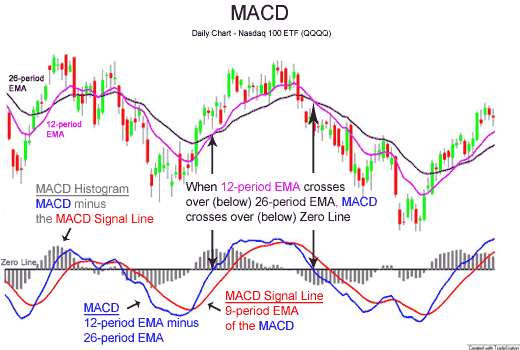
\includegraphics[width=0.6\linewidth]{macd}
\caption{Иллюстрация MACD с параметрами $l=26, s=12, a=9$\label{fig:macd}}
\end{figure}

На рисунке \ref{fig:macd} изображены примеры колебаний данных, их усреднения с периодами 12 и 26 (сверху) и разница этих средних,
ее усреднение с периодом 9 и их разность (снизу).


\subsection{Методика проведения сравнения стратегий}

Производится сравнение 2 стратегий. Обеим дается в начале периода одинаковая сумма денег, после чего:
\begin{itemize}
\item стратегия MACD реагирует на соответствующие сигналы и принимает решение, купить или продать предмет оборота
\item стратегия основанная на тестируемом классификаторе действует жадно, опираясь на его предсказание завтрашнего
поведения курса $y_{i+1}$
\end{itemize}
Обе стратегии ведут себя наивно-жадно, в каждой операции задействуя все имеющиеся средства для обмене.

Далее для каждого дня берется количество денежных средств, имеющихся у каждой из стратегий (если средства были
вложены в покупку, то они переводятся в денежный эквивалент по курсу этого дня). Для определения сравнительного состояния
стратегий на определенный день, рассматривается отношение их денежных средств: это удобный показатель, не зависящий
от текущего курса, а только от ``объема благ'', накопленных каждой стратегией.

Итак, если $a^{\text{ML}}_i, b^{\text{MACD}}_i$ --- денежные средства стратегий на день $i$, тогда для периода из $n$ дней
\begin{equation}
q_\text{macd} = \frac{\sum_i^n \frac{a^{\text{ML}}_i}{b^{\text{MACD}}_i}}{n}
\end{equation}

Таким образом, данную величину можно понимать как средний выигрыш по сравнению с торговлей по MACD.

\section{Линейные модели для предсказания}

Одними из самых простых, но в тоже время достаточно мощных моделей в машинном обучении являются линейные модели\cite{linear_cls}.
Для представления $x\in\mathcal{X}=(x^1,\ldots,x^m)$ обученный классификатора характеризуется вектором весов $w\in\mathbb{R}^m$,
и его предсказание получается как ($f(a) : \mathbb{R}\to\mathcal{Y}$ -- функция,
характеризующая подсемейство классификаторов)
\begin{equation}
y=f(w^Tx)
\end{equation}

Один из методов обучения данных классификаторов связан с представлением искомых $w^*$ как решения задачи минимизации
по обучающей выборке:
\begin{equation}
w^*=\argmin_w \sum_{i=1}^{|X|} L(y_i,w^Tx_i) + R(w)
\end{equation}

Выше
\begin{itemize}
\item $L(y_i, y)$ -- \textit{функция потерь}, оценивающая ошибки предсказания.
Важно, что она применяется к соответствующему $f(a)$. Примеры:
\begin{itemize}
\item log loss: $L(y_i, y) = -y_i\log{y}-(1-y_i)\log{(1-y)}$, $y$ имеет смысл предсказанной вероятности принадлежности
выделенному классу
\item hinge loss: $L(y_i, y) = \max(0, 1 - yy_i)$, здесь для удобства $y \in \{-1,1\}$.
\end{itemize}
\item $R(w)$ -- регуляризация\cite{regularization}, часть, предотвращающая деградацию качества на данных, на которых
алгоритм не обучался. Примеры ($\lambda_1,\lambda_2\geq0$):
\begin{itemize}
\item $L_2: R(w)=\lambda_2\|w\|_2$
\item $L_1: R(w)=\lambda_1\|w\|_1$
\item $L_1 + L_2: R(w)=\lambda_1\|w\|_1+\lambda_2\|w\|_2$
\end{itemize}
Последние 2 функции могут приводить к занулению некоторой части координат вектора $w^*$.
\end{itemize}

Наиболее распространенным в последнее время стало решение данной задачи с помощью SGD\cite{sgd}. 

\section{Векторизация текста}

Важным этапом для работы с любыми текстовыми источниками является процесс их векторизации --- представления их в векторном
виде. Будем считать, что нам дан текст на английском языке. Тогда одним из общепринятых методов перевода будет следующая
последовательность преобразований:
\begin{enumerate}
\item Токенизация\cite{info_retrieval}: для текста ``\texttt{About seven bits of important information is contained here!}'' получается
его разбиение на части, называемые токенами: (``\texttt{about}'', ``\texttt{seven}'', ``\texttt{bits}'', ``\texttt{of}'',
``\texttt{important}'', ``\texttt{information}'', ``\texttt{is}'', ``\texttt{contained}'', ``\texttt{here}'). Различные детали, как считать ли знаки препинания отдельными токенами, или переводить ли токены в 1 регистр, зависят от
токенизатора.
\item Лемматизация\cite{info_retrieval}: текстовые токены приводятся в ``нормальную форму'':
(``\texttt{about}'', ``\texttt{seven}'', ``\texttt{bit}'', ``\texttt{of}'',
``\texttt{important}'', ``\texttt{information}'', ``\texttt{be}'', ``\texttt{contain}'', ``\texttt{here}').
Это довольно нетривиальный процесс, не всегда существующие машинные техники получают результат, корректный с точки
зрения человека. Альтернативой является стемминг, при котором различные формы слова приводятся к одинаковому виду,
который необязательно является корректным словом.
\item Фильтрация стопслов: выбрасываются слова, не несущие самостоятельного смысла, например, артикли и местоимения:
(``\texttt{seven}'', ``\texttt{bit}'', ``\texttt{important}'', ``\texttt{information}'', ``\texttt{contain}'')
\item Дополнительная фильтрация слов: зачастую, происходит фильтрация по частоте встречаемости, для избавления от слишком редких
слов
\item Превращение текста в вектор: пусть для корпуса из $n$ текстов каждый прошел описанную выше обработку $w_i \in W,
w_i=(w_i^1,\ldots,w_i^{l_i})$ --- получившиеся последовательности, тогда классическое преобразование
полученной последовательности элементов $w_i$ в вектора Bag-of-Words\cite{info_retrieval}:
\begin{equation}
v\in\mathbb{R}^m: m=\left|\bigcup_{i,j} \{w^j_i\}\right|,\ v^j_i - \text{количество вхождения терма } j\text{ в } w_i
\end{equation}
\end{enumerate}

\section{Понижение размерности}

Зачастую при работе с большим количеством признаков, например, при работе с текстами, появляется желание уменьшить
размер признакового пространства без большой регрессии качества на данных. Одним из классических методов является
понижение размерности с помощью SVD\cite{svd}.

В нем признаковая матрица $X\in\mathbb{R}^{n\times m}$ представляется в виде $X=U\Sigma V^*$, где $\Sigma$ --- диагональная
матрица, где на диагонали расположены сингулярные значения матрицы упорядоченные по убыванию, а $U$ и $V$ --- матрицы 
соответствующих им левых и правых сингулярных векторов. Тогда можно показать, что для $X_m=U_m\Sigma_m V_m$,
где матрицы с индексов $m$ получены как подматрицы из элементов с индексами $i,j=\overline{1m}$,
$X_m$ является наилучшим приближением в смысле Фробеунисовой нормы ($\|A\|_F = \sqrt{\sum_{i,j} a^2_{ij}}$)
матрицы $X$ среди матриц ранга $m$.

Одним из преимуществ использования SVD является оценка потерь при понижения размерности, т.к. $\|Ax\|_2 \leq \|A\|_F\|x\|_2$,
и по доле суммы квадратов оставшихся сингулярных значений можно оценить величину потери для $Ax$, что важно для линейной
модели.

\chapter{Вычислительный эксперимент}

В качестве языков программирования в работе использовались C++ и Python\cite{python}.

\section{Данные}

\subsection{Данные новостей}

В качестве новостных данных были взяты новости из архива Reuters на английском языке за 2010-2017 годы\cite{reuters}. Датасет был получен с помощью робота, написанного с использованием библиотеки Scrapy\cite{scrapy}.

\subsection{Данные по торговому курсу}

В качестве примера цели прогнозирования были взяты изменения значения официального курса доллара к российскому рублю, доступные
на сайте Центрального Банка РФ\cite{courses}; так как этот курс формируется по среднему значению на период после начала торгов,
то его прогнозирование имеет практический смысл и может служить ориентиром для проведения торговых операций.
Официальный курс публикуется в 11:30 по московскому времени и действует на следующие календарные дни, до вступления в силу следующего
официального курса.

Официальный курс установлен не для всех дней (выпадают выходные, праздники и прочее).
Будем считать, что новость повлияла на курс дня, для которого известен курс и произошло следующее за ее публикацией 11:30.
Так как для практической применимости результатов требуется давать прогноз с запаздыванием, позволяющим провести торговые операции,
то целью предсказания мы будем считать изменение курса на день позже.

Другими словами, если $T_1,\ldots,T_n$ -- упорядоченная последовательность дней, для которых известен курс, то:
\begin{itemize}
\item новость, опубликованная в день $T_i$ ранее 11:30, участвует в прогнозировании для дня $T_{i+1}$
\item новость, опубликованная в день $T_i$ позднее 11:30, участвует в прогнозировании для дня $T_{i+2}$
\end{itemize}

Значение, которое требуется предсказать -- это знак изменения курса, таким образом задача сводится к бинарной классификации.

\subsection{Разбиение данных}

Разбиение на $X_\text{train}, X_\text{valid}, X_\text{test}$ было произведено в соотношении $2:2:1$.
Такие нетипично большие размеры валидационной и тестовых частей были вызваны необъективностью показателя
$q_\text{macd}$ на малых отрезках, из-за чего и потребовалось выделить для каждой из них значительную часть выборки.

\section{Обработка текстовых данных}

\subsection{Векторизация новостей}

Этапы векторизации текста новостей, для первых 2 этапов была использована их реализация в библиотеке NLTK\cite{nltk}:

\begin{enumerate}

\item Токенизация. Был использован известный метод Treebank\cite{treebank}) с последующим отсеиванием токенов,
содержащих символы кроме буквено-цифровых.
\item Лемматизация. Использовался WordNet\cite{wordnet}, из-за специфики статей результаты были вполне удовлетворительными,
и было решено использовать их, а не результаты стемминга.
\item Учет \texttt{not} и стоп-слова. Было решено произвести фильтрацию стоп-слов, однако до этого последовательности
термов (\texttt{not}, $w_1$, $w_2$) были заменены на ($\text{not\_} w_1, \text{not\_} w_2$) для учета смыслового отрицания
для прилагательных.
\item Добавление биграмм\footnote{пара термов, идущих подряд в тексте} как самостоятельных термов.
\item Частотная фильтрация --- оставить термы со встречаемостью не менее 10000 на весь корпус. В дальнейшем было проверено,
что множество оставшихся термов не уменьшается при уменьшении выборки на 25\%, что позволяет сказать об устойчивости
результата для данного формата данных. В среднем на каждый день приходится 1200 статей.

\end{enumerate}

В результате осталось около 7000 термов, после чего было использовано стандартное представление Bag-of-Words.

\subsection{Сведение от новостей к дням}

Так как прогнозирование делается для дней, то необходимо получить векторное представление дня.
В данной работе был использован один из самых очевидных способов, а именно представлять вектор дня как сумму векторов соответствующих этому дню новостей, деленную на их количество.
\begin{equation}
x_i = \frac{1}{\left|\{v_j | time(v_j)=T_i\}\right|} \sum_{v_j: t(v_j)=T_i} v_j
\end{equation}

\section{Преобразование признаков}

После понижения размерности с помощью SVD\cite{svd} с сохранением
99\% информации количество оставшихся фич составило 1700, что позволило решать задачу с использованием стандартных
приемов регуляризации. С получившейся матрицей было произведено попризнаковое
масштабирование: для каждого значения признака из него было вычтено его среднее значение по выборке и результат поделен на
выборочное отклонение.

\section{Результаты}

Итоговый линейный классификатор был обучен с помощью SGD\cite{sgd}, параметры регуряризации ($\lambda_1,\lambda_2$ для L1+L2)
и целевая функция (log-loss, hinge-loss) выбирались на кроссвалидации.

На рисунке \ref{fig:vs_macd_on_test} приведен график для 3 классификаторов, численное сравнение в таблице \ref{test_table_compare}:

\begin{itemize}
\item \texttt{Top accuracy} -- классификатор с гиперпараметрами с лучшим значением $q_\text{acc}$ на кроссвалидации,
\item \texttt{Top trade} -- классификатор с гиперпараметрами с лучшим значением $q_\text{macd}$ на кроссвалидации,
\item \texttt{Combine} -- классификатор с гиперпараметрами с максимальным значением $R(q_\text{acc}) + R(q_\text{macd})$ на кроссвалидации,
где $R(\cdot)$ --- ранг, порядковый номер элемента в последовательности значений гиперпараметров, упорядоченной по возрастанию
соответствующей метрики качества;
\end{itemize}

\begin{figure}[h]
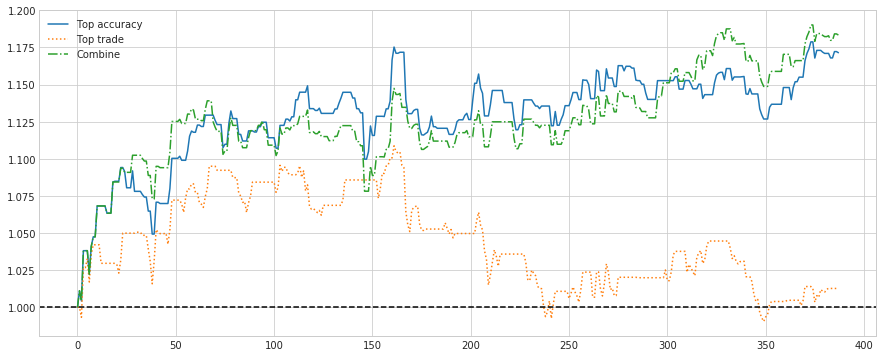
\includegraphics[width=\linewidth]{vs_macd_on_test}
\caption{Поведение торговых стратегий по сравнению с MACD на тестовой выборке \label{fig:vs_macd_on_test}}
\end{figure}

\begin{table}[h]
\centering 
\begin{tabular}{| c | c | c |}
\hline
 & Среднее & Отклонение \\ \hline
Top trade & 1.04 & 0.030 \\ \hline
Top accuracy & 1.13 & 0.029 \\ \hline
Combine & 1.13 & 0.031 \\ \hline
\end{tabular}
\caption{Выборочные статистики отношения стратегий к MACD на тестовой выборке\label{test_table_compare}}
\end{table}

Как можно увидеть, лидером является классификатор с максимальной точностью, но смешанная версия не сильно проседает по качеству,
причем на отдельных отрезках опережает остальные. В целом, результаты показывают, что полученный метод дает значимое преимущество перед стратегией, использующей MACD (горизонтальный уровень со значением 1).	

Также была проверена гипотеза о зависимости прогнозирования от какого-либо периода (дни недели, начало месяца и проч.).
Стандартный для этого тест Льюнг-Бокса\cite{ljungbox} для индикаторов истинности предсказаний на тестовой выборке
показал $p$-значение 0.88, что позволяет уверенно заключить об отсутствии автокорреляции.

\chapter{Итоги}

Таким образом, в данной работе на примере колебаний курса
валюты была продемонстрирована возможность прогнозирования финансовых показателей, основываясь исключительно на текстово-новостной информации.
Более того, была также произведена демонстрация его применения для создания торговой стратегии,
которая выигрывает в сравнении с классической экономической стратегией MACD.

Несмотря на то, что выигрыш над MACD был достигнут, целью данной работы в большей степени являлась иллюстрация
возможности такого предсказания, а не получение максимальной прибыли над MACD ценой узконаправленных эвристик,
из-за чего в продемонстрированном решении оставлено огромное поле для доработок.
На примере уже существующих работ в данной области для улучшения качества работы можно порекомендовать
смешение текстовых признаков и признаков, описывающих численное поведение курса за небольшую историю;
также нераскрытой остается возможность выделения для новостей признаков, связанных с поведением курса, и изменением
способа представления дня на их основе.

Используемые методы не привязаны к специфике курсов валют, позволяя использовать их для прогнозирования других
финансовых показателей.

\bibliography{literature}{}
\bibliographystyle{plain}

\end{document}
